\section{Twilio Overview}
\label{sec-twilioecoandprotocolstudy}
In what follows, we describe the Twilio Ecosystem, the high level protocol study and the message level protocol study.
\subsection{Twilio Ecosystem}
\label{subsec-twilioeco}
The twilio ecosystem, as depicted in the Figure~\ref{fig:ecosystem} can be viewed as a layered architecture. In the bottom most layer sits the $Twilio$  $Servers$. These servers exposes a set of data and voice communication APIs for sending and receiving voice calls and messages. In the middle layer lies the $Application$ $Servers$. These servers are installed by Twilio customers with Twilio accounts. For e.g. These application servers might belong to some company X who want to provide VoIP service to its customer.  

Each Twilio account is linked to a 1) Twilio number 2) Account SID 3) Auth Token. A Twilio number is ten digit phone number. Account SID is unique identifier for a Twilio account. Auth Token is a token used by Twilio Servers to authenticate Application servers. The Application server uses the Account SID and Auth Token to access the Twilio APIs. The cost model for Application servers is typically pay per message or pay per call. On the top most layer are the Clients which could be browser based client or phone based clients. For e.g. These clients could be the customers of company X who is providing VoIP service. These clients can be free customers or paid customers of company X. The Clients in order to use the service and communicate with each other need to register with the Twilio Server. This is done using a capability token which is provided by the Application Server. 
\begin{figure}
\centering
%\begin{minipage}{.45\textwidth}
  \centering
  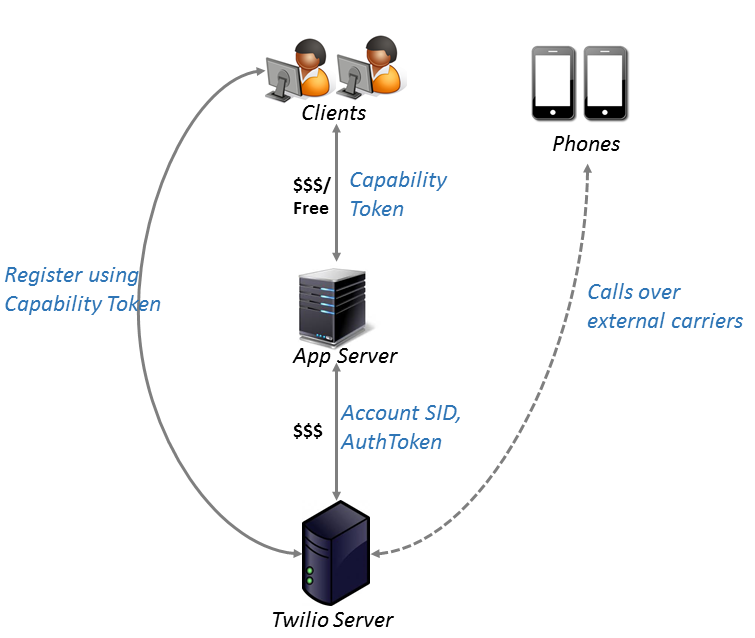
\includegraphics[width=0.45\textwidth]{figs/Ecosystem.png}
  %Mazu_frame_new.png}
\caption{Twilio Ecosystem}
\label{fig:ecosystem}
\end{figure}     

\emph{Application Container: } Each Twilio number is linked to a application container. The application container contains two URLS: Voice URL and Message URL. These URLs are configurable and are configured by the App Server administrators (Twilio customers). Whenever a incoming call or meesages for a Twilio number arrives, the Twilio server makes a post request on these URLs. The content generated by these URLs direct Twilio Server to perform the needed actions on those incoming calls or messages. These contents are in form of a special markup language called $TwiML$.

\emph{TwiML:  } TwiML is a markup language developed by Twilio. It is a set of instructions in form of verbs that can be used by the Application Servers to tell Twilio what to do when a call or message is received to its number. Various kinds of verbs are supported as shown below which can be used to create interactive applications atop Twilio.
\begin{itemize}
\item  Say - Read text to the caller 
\item Play - Play an audio file for the caller
\item Dial - Add another party to the call
\item Record - Record the caller's voice
\item Gather - Collect digits the caller types on their keypad
\item Sms - Send an SMS message during a phone call
\item Hangup - Hang up the call
\item Queue - Add the caller to a queue of callers.
\item Redirect - Redirect call flow to a different TwiML document.
\item Pause - Wait before executing more instructions
\item Reject - Decline an incoming call without being billed.
\end{itemize}

For e.g. The TwiML snippet shown in Figure~\ref{fig:TwilML} will say Hello World to the caller.
 
\begin{figure}
\centering
%\begin{minipage}{.45\textwidth}
  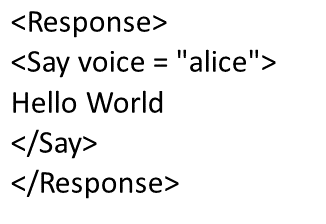
\includegraphics[width=0.25\textwidth]{figs/TwiML.png}
\caption{Sample TwiML Snippet}
\label{fig:TwilML}
\end{figure} 

\begin{figure*}[t!] 
\centering
%\begin{minipage}{.45\textwidth}
  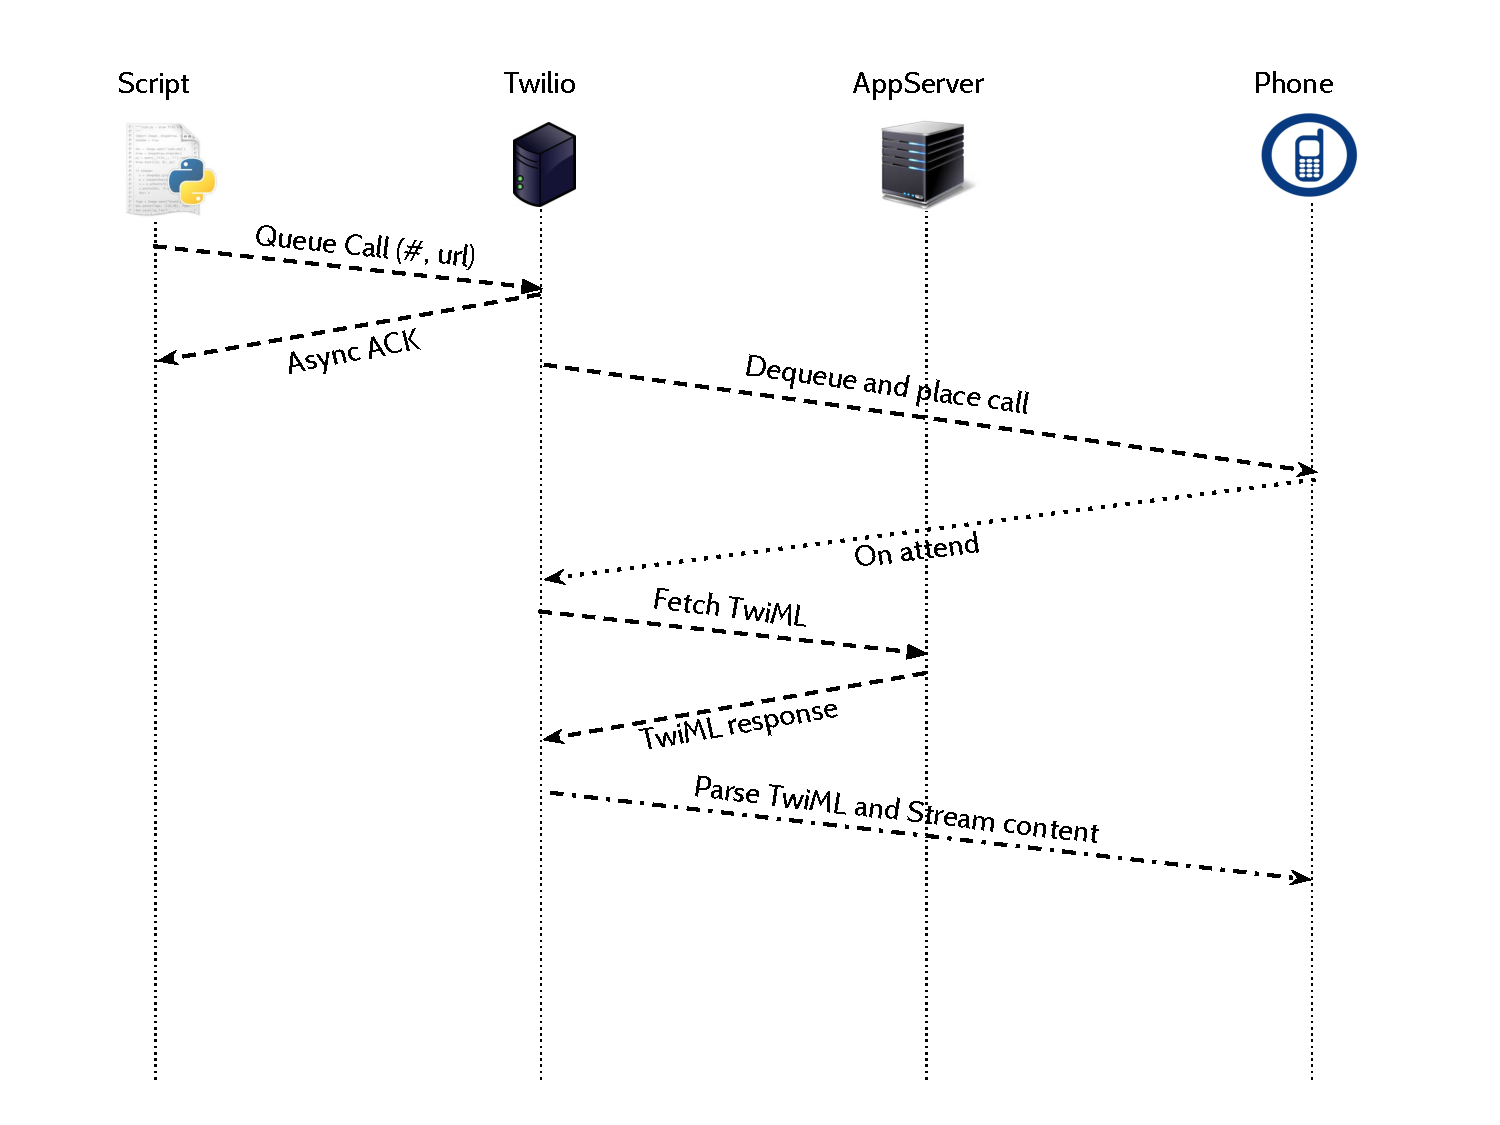
\includegraphics[width=0.8\textwidth]{figs/auto.pdf}
\caption{Automated call to a phone}
\label{fig:autocall}
\end{figure*} 

\subsection{Scenarios}

There are multiple scenarios possible with the help of Twilio Apis. It include:

\begin{itemize}
\item Automated Calls
\item Voice Calls
\begin{itemize}
\item Phone to VoIP Client
\item VoIP Client to Phone
\item VoIP Client to VoIP Client
\end{itemize}
\item Messages
\end{itemize}

\subsection{Experimental Setup}

We developed a simple VoIP service called VoT atop Twilio and deployed it in OpenShift RedHat Cloud. The VoT server also hosts a website which is used to place voice calls. For making automated calls and sending automated messages we have developed some python scripts which directly calls into the Twilio APIs. For our study we extensively use traces collected at different places. This includes application level trace messages in VoT, logs in Twilio user portal, Twilio object store queries and wireshark traces in client machines.

\subsection{High Level Protocol Study}

We now present a high level protocol study of various scenarios that Twilio supports. 

\emph{\textbf{Automated calls to phones:} }
The protocol diagram for this scenario is shown in  Figure~\ref{fig:autocall}. At first the script places a call queue request specifying the phone number to which the call needs to be placed and a url where the message located. The Twilio server acknowledges the request and places the call. Once the phone attends the call, the Twilio server uses the url in the call queue request to contact the Application server and request the content (in form of TwiML) that needs to be delivered to the phone. The Application server processes the request and sends a TwiML response. The Twilio server parses the TwiML and streams the content to the phone.  


\emph{\textbf{Voice calls between VoIP clients:} }
\begin{figure*}[t!] 
\centering
%\begin{minipage}{.45\textwidth}
  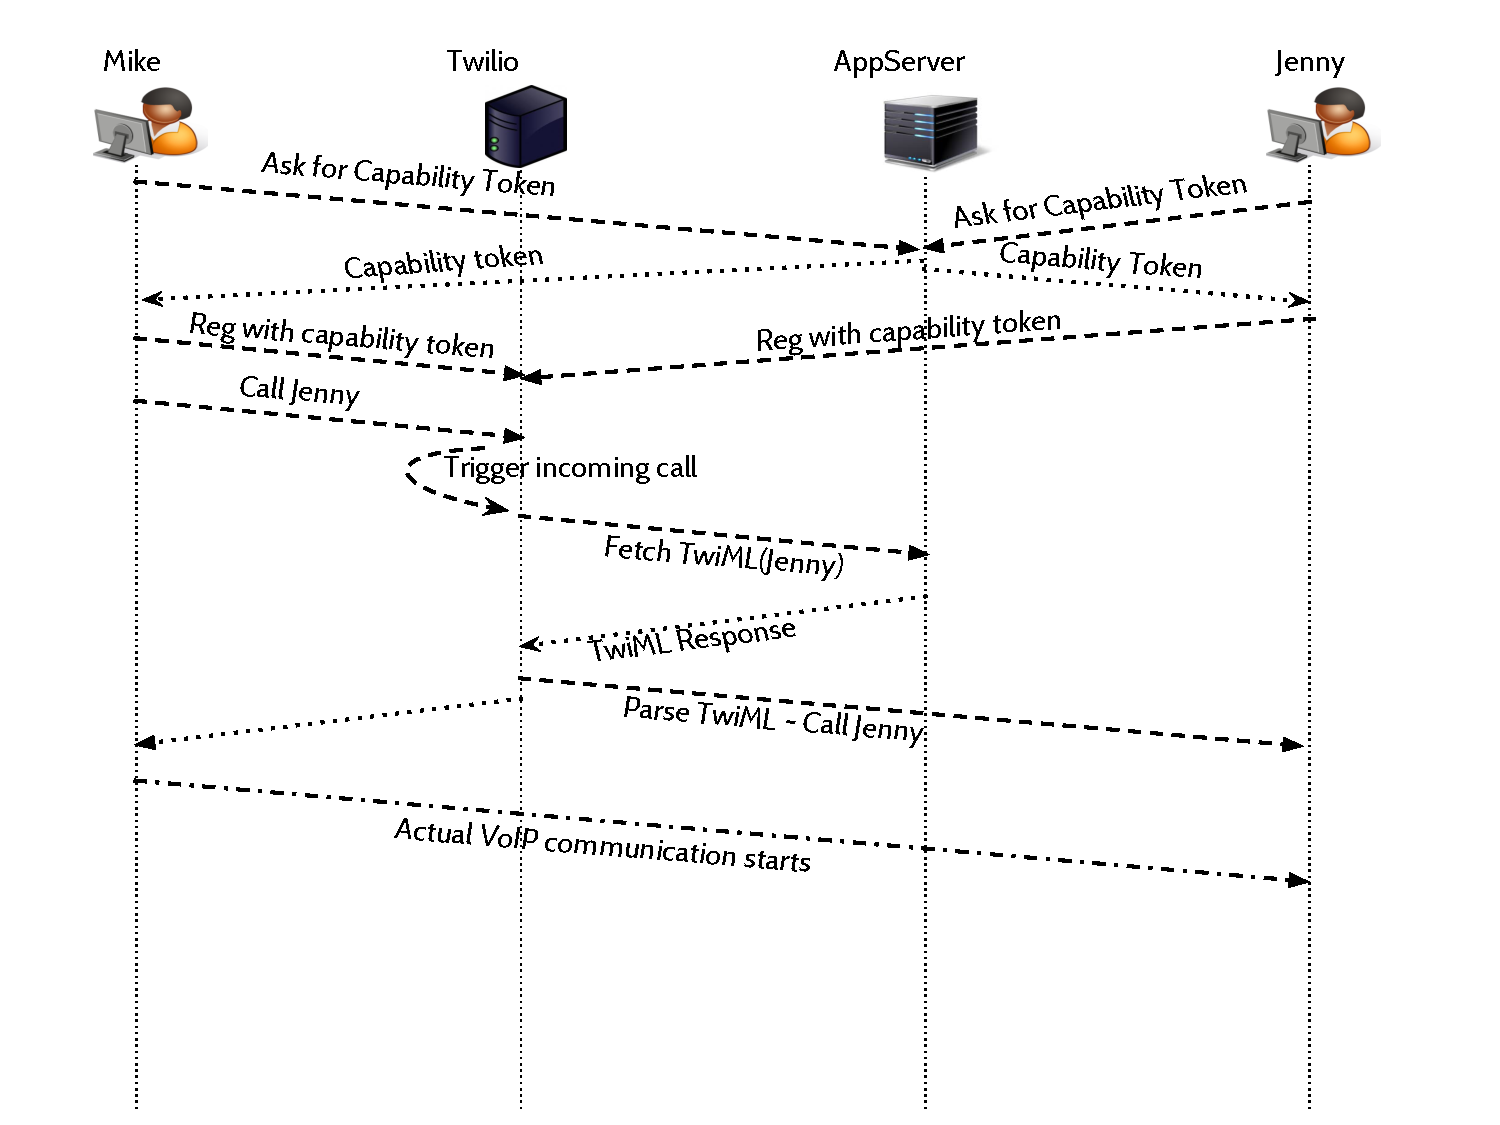
\includegraphics[width=0.8\textwidth]{figs/twoclients.pdf}
\caption{Call between two VoIP clients}
\label{fig:2VoIPcall}
\end{figure*}
The protocol diagram for this scenario is shown in Figure~\ref{fig:2VoIPcall}. Lets say, Mike and Jenny are the two VoIP clients and Mike wish to call Jenny. As shown in Section~\ref{subsec-twilioeco}, for Mike and Jenny to communicate they need to first register with the Twilio Server. Hence, Mike and Jenny at first request the Application server for capability tokens. Once the Application server delivers the tokens, Mike registers with the Twilio server using the token. Mike then queues a call to Jenny. An interesting thing to note here is that the Twilio server does not have information about what to do with the call. It has to communicate with the Application server to get this information. For this, it triggers an incoming call to the Twilio number linked with Mike. As shown in Section~\ref{subsec-twilioeco}, every incoming call generates a post request on the voice URL present in the application container. This post request is directed to the Application server with query parameter as "Jenny". The Application server parses the request and the query parameter, generates the appropriate TwiML content for the action that needs to be taken and delivers it to the Twilio server. The Twilio Server parses the TwiML and places a call to Jenny. Finally, Mike is notified about this and the actual communication starts. 

\emph{\textbf{Voice calls from VoIP clients to phone:} }
The protocol diagram for this scenario is similar to that shown in Figure~\ref{fig:2VoIPcall} except Jenny has a dedicated phone number and does not need to register with the Twilio server. Lets say, Mike is a VoIP client and Mike wish to call Jenny's phone. Mike will at first request the Application server for a capability token. Once the Application server delivers the token, Mike will register with the Twilio server. Mike then queues a call to Jenny. As in the case of two VoIP clients in the previous section, the Twilio server does not have information about what to do with the call. It has to communicate with the Application server to get this information. For this, it triggers an incoming call to the Twilio number linked with Mike. This incoming call generates a post request on the voice URL present in the application container. This post request is directed to the Application server with query parameter as "Jenny's phone number". The Application server parses the request and the query parameter, generates the appropriate TwiML content for the action that needs to be taken and delivers it to the Twilio server. The Twilio Server parses the TwiML and places a call to Jenny's phone. Finally, Mike is notified about this and the actual communication starts.
 
\emph{\textbf{Voice calls from phone to VoIP clients:} }
\begin{figure*}[t!] 
\centering
%\begin{minipage}{.45\textwidth}
  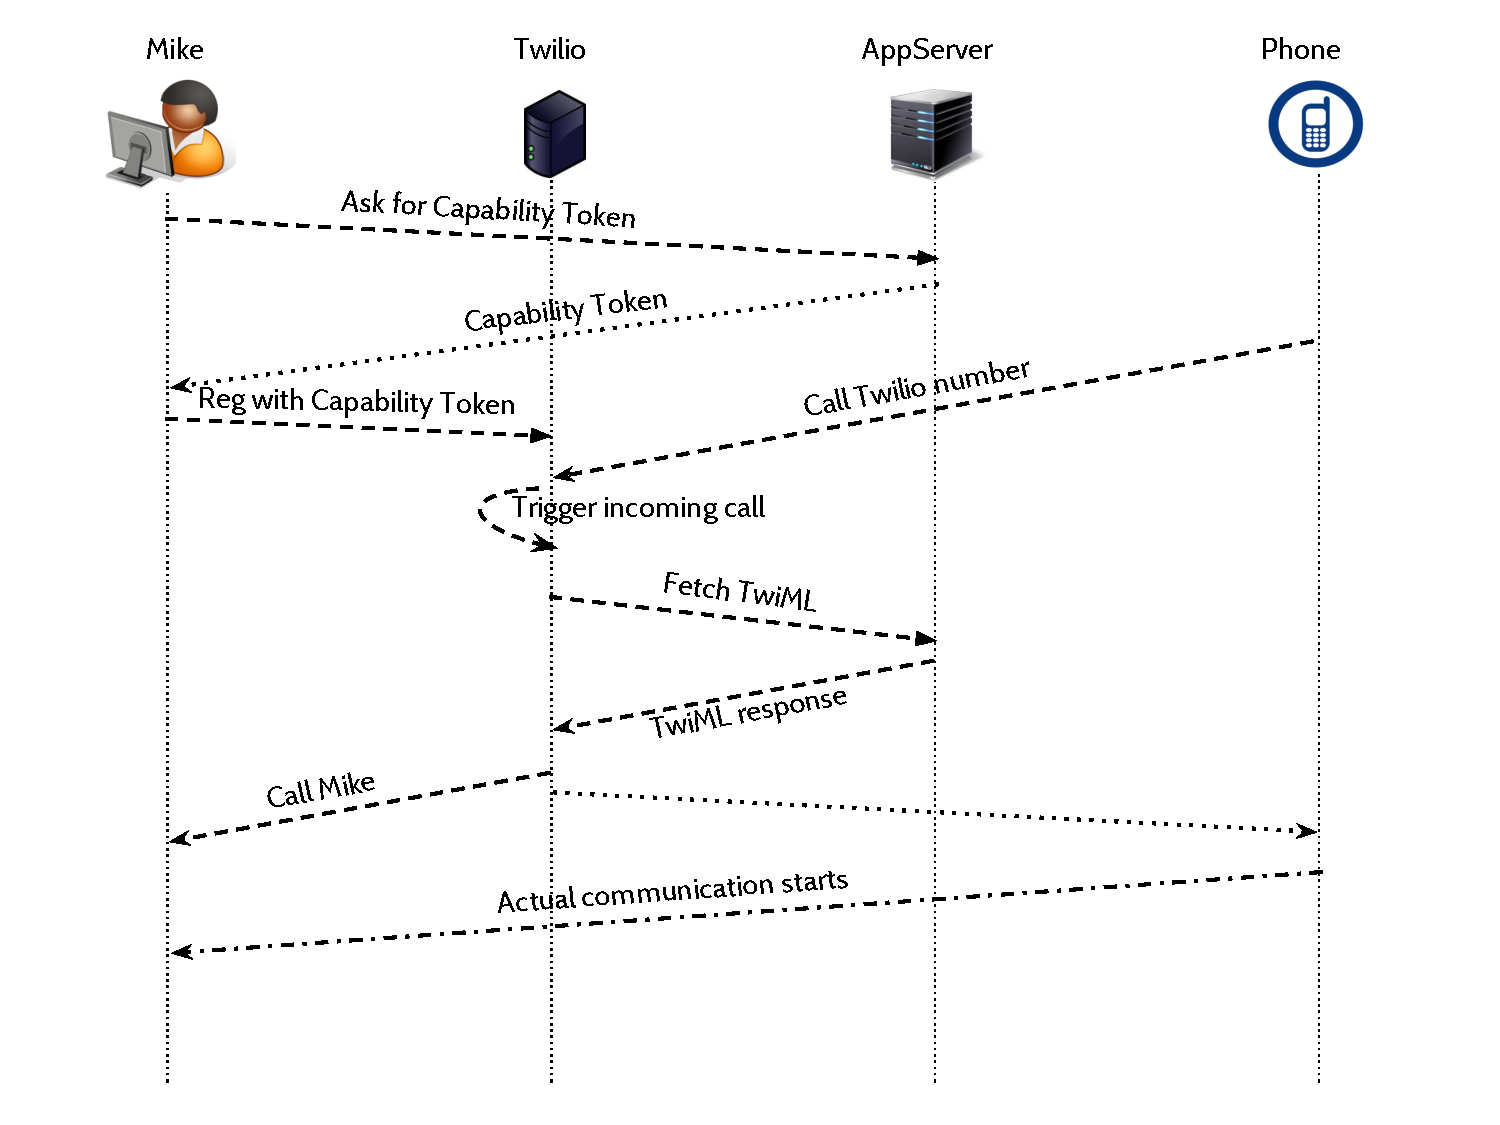
\includegraphics[width=0.8\textwidth]{figs/p2c.pdf}
\caption{Call from phone to a VoIP client}
\label{fig:callfromphone}
\end{figure*}
The protocol diagram for this scenario is shown in Figure~\ref{fig:callfromphone}. Lets say, Mike be the VoIP client and a phone wish to call Mike. Mike will first request the Application server for capability token. Once the Application server delivers the token, Mike registers with the Twilio server. When the phone calls the Twilio number associated with Mike, the Twilio server triggers an incoming call to the Twilio number. The incoming call generates a post request on the voice URL present in the application container. This post request is directed to the Application server. The Application server parses the request, generates the appropriate TwiML content for the action that needs to be taken and delivers it to the Twilio server. The Twilio Server parses the TwiML and places a call to Mike. Finally, the phone is notified about this and the actual communication starts.

\subsection{Packet Level Analysis}
In this subsection, we present the packet level analysis for a scenario when a browser make a voice call to a phone or another browser based client. We also show one more message level analysis for automated message sending scenario in section \ref{sec-oddities}. 

\begin{figure*}[t!] \centering
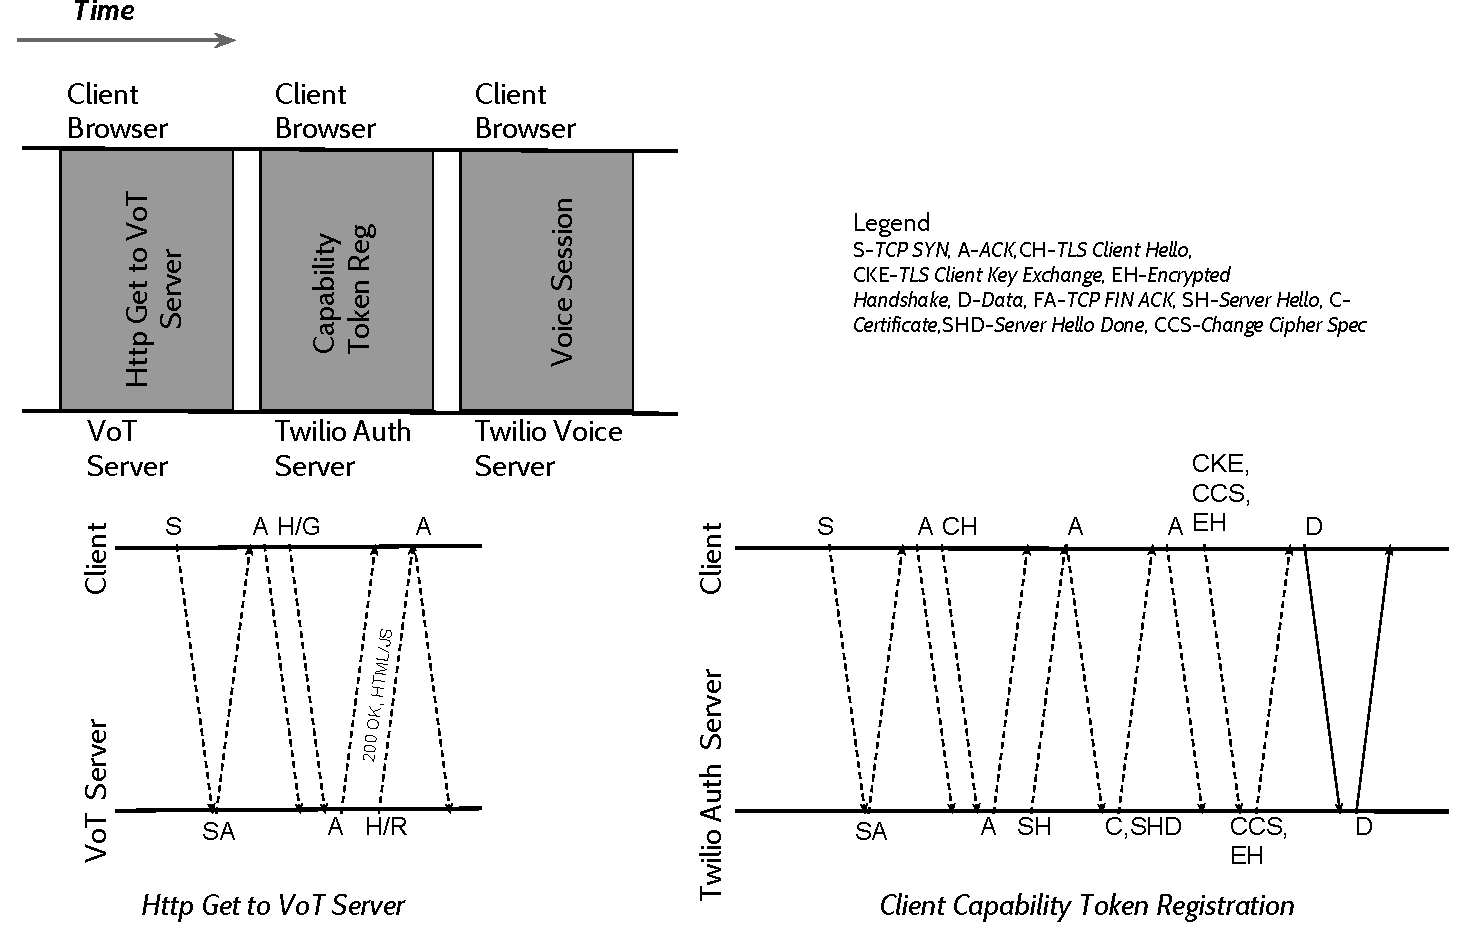
\includegraphics[width=\textwidth]{figs/voicecallpacketlevel.pdf}
\caption{\textbf{Voice Call from Browser Client} {\footnotesize\textit{
The figure shows sequence of packet exchanges that happen between the client and other components of the system. The top diagram shows the high level operations. The participants are shown above and below the top and bottom lines. The left bottom figure shows how the client interacts with the application server to obtain the \textit{capability token} and it corresponds to the first block in the top diagram. The right bottom diagram shows the sequence of messages exchanged between the client and the \textit{Twilio} server when the client executes the \textit{Twilio.Device.Setup} method and corresponds to the second block in the top diagram.  
}}}
\label{fig:messagelevel}
\end{figure*}

Figure~\ref{fig:messagelevel} shows the sequence of event that happens when a browser based client wants to make a VoIP call to another browser based client or another phone. As shown, at first the client browser does a \textit{HTTP GET} request to the application server that we have deployed. The application server generates a \textit{capability token} and passes it onto the client. The client side javascript includes the \textit{twilio js} library and does \textit{Twilio.Device.Setup} to register its capability with the \textit{Twilio} servers. The sequence of messages for the second block is also shown. The client passes the \textit{token} as \textit{HTTP} data after establishing a TLS session with the server. After this step, the client is free to make a call to either another browser based client or another phone number. The actual voice communication is tunneled through \textit{Twilio} servers and it involved \textit{RTMP} protocol. This sequence of packet exchanges are not shown due to space constraints. 
